\chapstart
\section{THIẾT KẾ CƠ SỞ DỮ LIỆU}
\label{sec:database-design}
\begingroup
\setlist[itemize]{leftmargin=1.27cm,label=\textbullet,itemsep=2pt,topsep=4pt}
\setlist[enumerate]{leftmargin=1.27cm,itemsep=2pt,topsep=4pt}
\setlength{\emergencystretch}{1em}
\widowpenalty=10000
\clubpenalty=10000

BroomSharing sử dụng database \texttt{broomsharing} của Cloud Firestore để lưu dữ liệu tài khoản, không gian, đặt chỗ và trao đổi giữa các bên. Firebase Authentication quản lý danh tính đăng nhập, liên kết với hồ sơ người dùng qua UID. Cloudinary lưu ảnh và minh chứng DEMO, còn Firestore giữ URL tham chiếu. Backend Java quản lý giao dịch payOS và trạng thái tiền \parencite{broomsharing_source}.

\subsection{Các thực thể và thuộc tính}
\label{sec:ch4-entities}

Dữ liệu ứng dụng được tổ chức thành 17 collection gốc và ba loại subcollection, tương ứng 20 mẫu document đang được ứng dụng hoặc backend sử dụng trong Bảng~\ref{tab:ch4-entities-summary}. Các thuộc tính định danh liên kết tài khoản với tài sản và yêu cầu thuê; nhóm trạng thái chi phối việc công bố phòng, xét duyệt và chuyển bước đặt chỗ. Collection thông báo cũ chỉ còn contract trong Rules, không phải nguồn hộp cập nhật đang hoạt động. Document còn chứa dữ liệu nhúng dạng \texttt{map}, \texttt{array} và các mốc thời gian xử lý. Những trường như người duyệt hoặc thời điểm hủy chỉ phát sinh khi nghiệp vụ tương ứng được thực hiện.

\begingroup\small\setstretch{1.06}
\begin{longtable}{@{}>{\raggedright\arraybackslash}p{3.6cm}>{\raggedright\arraybackslash}p{3.75cm}>{\raggedright\arraybackslash}p{7.9cm}@{}}
\caption{Các mẫu document và thuộc tính tiêu biểu}\label{tab:ch4-entities-summary}\\
\toprule Đường dẫn & Vai trò & Thuộc tính tiêu biểu và kiểu \\ \midrule\endfirsthead
\toprule Đường dẫn & Vai trò & Thuộc tính tiêu biểu và kiểu \\ \midrule\endhead
\midrule\multicolumn{3}{r}{\small Còn tiếp ở trang sau}\\\endfoot
\bottomrule\endlastfoot
\texttt{users/\allowbreak{}\{\allowbreak{}uid\}} & Hồ sơ và quyền tài khoản. & \texttt{uid}, \texttt{role}, \texttt{status}, \texttt{photo\allowbreak{}Url} (\texttt{string}); \ldots \\
\texttt{public\allowbreak{}Hosts/\allowbreak{}\{\allowbreak{}uid\}} & Bản chiếu Host. & \texttt{uid}, \texttt{name}, \texttt{photo\allowbreak{}Url} (\texttt{string}); \ldots \\
\texttt{usernames/\allowbreak{}\{\allowbreak{}normalized\allowbreak{}Username\}} & Ánh xạ đăng nhập. & \texttt{uid}, \texttt{email} (\texttt{string}). \\
\texttt{host\allowbreak{}Applications/\allowbreak{}\{\allowbreak{}uid\}} & Đơn cấp quyền Host. & \texttt{applicant\allowbreak{}Uid}, \texttt{status} (\texttt{string}); \texttt{identity\allowbreak{}Image\allowbreak{}Urls} (\texttt{array\textless{}\allowbreak{}string\textgreater{}}); \ldots \\
\texttt{users/\allowbreak{}\{\allowbreak{}uid\}\allowbreak{}/\allowbreak{}favorites/\allowbreak{}\{\allowbreak{}room\allowbreak{}Id\}} & Phòng yêu thích. & \texttt{room\allowbreak{}Id}, \texttt{room\allowbreak{}Name} (\texttt{string}); \texttt{created\allowbreak{}At} (\texttt{timestamp}). \\
\texttt{users/\allowbreak{}\{\allowbreak{}uid\}\allowbreak{}/\allowbreak{}notice\allowbreak{}Reads/\allowbreak{}\{\allowbreak{}event\allowbreak{}Id\}} & Mốc đọc sự kiện dẫn xuất. & \texttt{read\allowbreak{}At} (\texttt{timestamp}). \\
\texttt{buildings/\allowbreak{}\{\allowbreak{}building\allowbreak{}Id\}} & Địa điểm và chủ sở hữu. & \texttt{owner\allowbreak{}Uid}, \texttt{name}, \texttt{address} (\texttt{string}); \texttt{location} (\texttt{geopoint/\allowbreak{}null}); \ldots \\
\texttt{rooms/\allowbreak{}\{\allowbreak{}room\allowbreak{}Id\}} & Không gian và trạng thái tin. & \texttt{building\allowbreak{}Id}, \texttt{owner\allowbreak{}Uid}, \texttt{active\allowbreak{}Mode} (\texttt{string}); \texttt{active\allowbreak{}Booking\allowbreak{}Count} (\texttt{integer}); \ldots \\
\texttt{bookings/\allowbreak{}\{\allowbreak{}booking\allowbreak{}Id\}} & Kỳ thuê, trạng thái và giá đã chốt. & \texttt{room\allowbreak{}Id}, \texttt{guest\allowbreak{}Uid}, \texttt{status}, \texttt{payment\allowbreak{}Flow} (\texttt{string}); \texttt{price\allowbreak{}Snapshot} (\texttt{map}); \ldots \\
\texttt{availability\allowbreak{}Months/\allowbreak{}\{\allowbreak{}room\allowbreak{}Id\_\allowbreak{}yyyy\allowbreak{}MM\}} & Khóa lịch chính thức và tạm giữ. & \texttt{fixed\allowbreak{}Booking\allowbreak{}Id} (\texttt{string}); \texttt{slots\allowbreak{}Busy} (\texttt{array\textless{}\allowbreak{}integer\textgreater{}}); \texttt{hourly\allowbreak{}Bookings} (\texttt{map\textless{}\allowbreak{}string,\allowbreak{}array\textless{}\allowbreak{}integer\textgreater{}\allowbreak{}\textgreater{}}); \texttt{pending\allowbreak{}Payment\allowbreak{}Ids} (\texttt{array\textless{}\allowbreak{}string\textgreater{}}); \ldots \\
\texttt{payments/\allowbreak{}\{\allowbreak{}booking\allowbreak{}Id\}} & Giao dịch trả trước. & \texttt{order\allowbreak{}Code}, \texttt{amount}, \texttt{expires\allowbreak{}At} (\texttt{integer}); \texttt{status} (\texttt{string}); \ldots \\
\texttt{payment\allowbreak{}Orders/\allowbreak{}\{\allowbreak{}order\allowbreak{}Code\}} & Ánh xạ mã đơn của backend. & \texttt{booking\allowbreak{}Id} (\texttt{string}). \\
\texttt{app\allowbreak{}Config/\allowbreak{}payments} & Cấu hình kênh demo công khai. & \texttt{flow}, \texttt{demo\allowbreak{}Host\allowbreak{}Uid} (\texttt{string}). \\
\texttt{reviews/\allowbreak{}\{\allowbreak{}booking\allowbreak{}Id\}} & Đánh giá sau sử dụng. & \texttt{room\allowbreak{}Id}, \texttt{guest\allowbreak{}Uid}, \texttt{comment} (\texttt{string}); \texttt{rating} (\texttt{integer}); \ldots \\
\texttt{conversations/\allowbreak{}\{\allowbreak{}guest\allowbreak{}Uid:host\allowbreak{}Uid\}} & Hội thoại và mốc đọc. & \texttt{member\allowbreak{}Uids} (\texttt{array\textless{}\allowbreak{}string\textgreater{}}); \texttt{sequence}, \texttt{guest\allowbreak{}Read}, \texttt{host\allowbreak{}Read} (\texttt{integer}); \ldots \\
\texttt{conversations/\allowbreak{}\{\allowbreak{}guest\allowbreak{}Uid:host\allowbreak{}Uid\}\allowbreak{}/\allowbreak{}messages/\allowbreak{}\{\allowbreak{}message\allowbreak{}Id\}} & Tin nhắn của hội thoại. & \texttt{sender\allowbreak{}Uid}, \texttt{text} (\texttt{string}); \texttt{sequence} (\texttt{integer}); \texttt{created\allowbreak{}At} (\texttt{timestamp}); \ldots \\
\texttt{property\allowbreak{}Verifications/\allowbreak{}\{\allowbreak{}verification\allowbreak{}Id\}} & Minh chứng xác minh. & \texttt{owner\allowbreak{}Uid}, \texttt{verification\allowbreak{}Type}, \texttt{status} (\texttt{string}); \texttt{evidence\allowbreak{}Refs} (\texttt{array\textless{}\allowbreak{}string\textgreater{}}); \ldots \\
\texttt{reports/\allowbreak{}\{\allowbreak{}report\allowbreak{}Id\}} & Phản ánh và kết quả xử lý. & \texttt{reporter\allowbreak{}Uid}, \texttt{room\allowbreak{}Id}, \texttt{booking\allowbreak{}Id}, \texttt{status} (\texttt{string}); \ldots \\
\texttt{audit\allowbreak{}Logs/\allowbreak{}\{\allowbreak{}audit\allowbreak{}Id\}} & Dấu vết thay đổi. & \texttt{actor\allowbreak{}Uid}, \texttt{target\allowbreak{}Path}, \texttt{action} (\texttt{string}); \texttt{before}, \texttt{after} (\texttt{map\textless{}\allowbreak{}string,\allowbreak{}any\textgreater{}}); \ldots \\
\texttt{rental\allowbreak{}Places/\allowbreak{}\{\allowbreak{}place\allowbreak{}Id\}} & Địa điểm tham khảo, không đặt thuê. & \texttt{name}, \texttt{source\allowbreak{}Url} (\texttt{string}); \texttt{location} (\texttt{geopoint}); \ldots \\
\end{longtable}\endgroup


Mô hình tách hồ sơ tài khoản khỏi bản chiếu Host, thông tin phòng khỏi lịch giữ chỗ và nội dung hội thoại khỏi từng tin nhắn. Các lớp tổng hợp phục vụ giao diện như \texttt{Room\allowbreak{}Listing}, \texttt{Booking\allowbreak{}Notice} và \texttt{Host\allowbreak{}Stats} không có collection độc lập. Trong booking, tên phòng, liên hệ người thuê và giá được lưu tại thời điểm đặt, duy trì ngữ cảnh của yêu cầu khi dữ liệu gốc thay đổi.

\subsection{Quan hệ dữ liệu và cấu trúc lưu trữ}
\label{sec:ch4-relationships}

Hình~\ref{fig:ch4-overview} thể hiện cây lưu trữ của hệ thống. Hai subcollection \texttt{favorites}, \texttt{notice\allowbreak{}Reads} thuộc từng document người dùng; \texttt{messages} thuộc từng document hội thoại. Các collection \texttt{buildings}, \texttt{rooms}, \texttt{bookings} và \texttt{availability\allowbreak{}Months} nằm ngang cấp, liên kết bằng các trường ID dạng chuỗi. Cấu trúc phân cấp này tuân theo mô hình collection và document của Firestore \parencite{firebase_data_model}.

% Original Page-2 through Page-6. Full vector figures; no redrawing/cropping.
\begin{figure}[H]
\centering
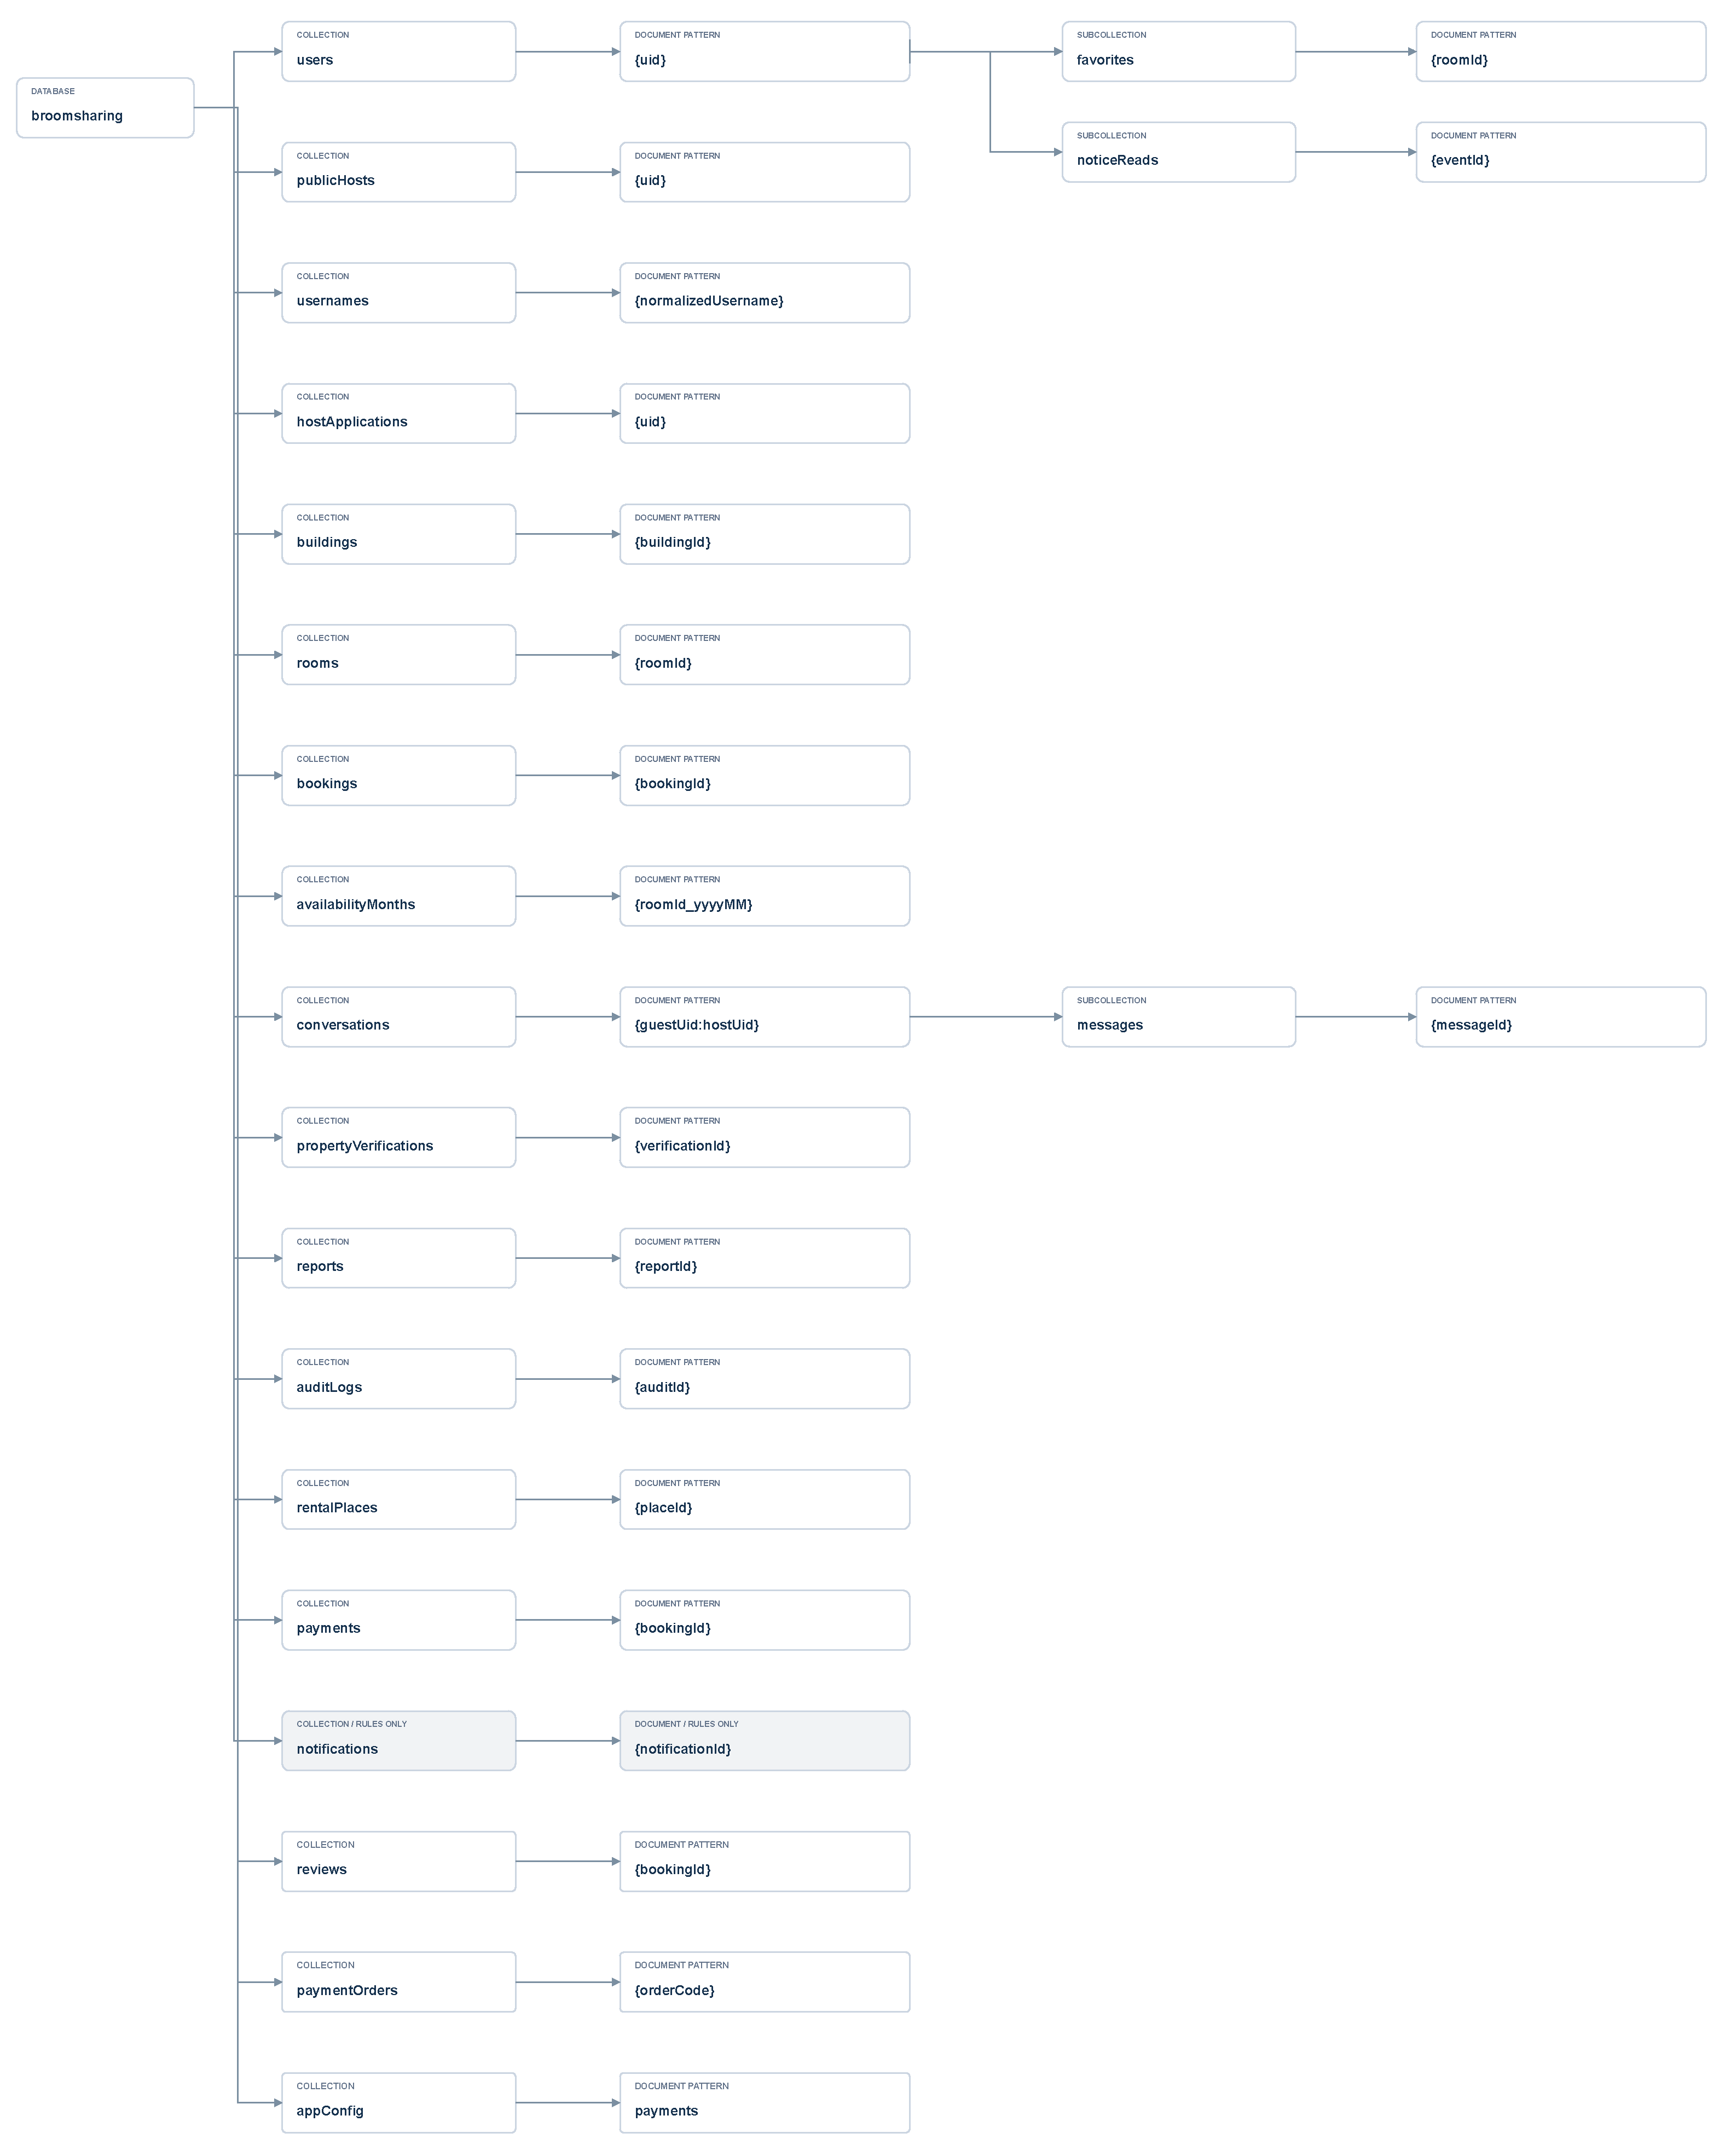
\includegraphics[width=\textwidth,height=0.86\textheight,keepaspectratio]{chapter4/firestore-overview.pdf}
\caption{Cây lưu trữ Firestore BroomSharing. Thẻ màu xám là contract thông báo cũ trong Rules.}
\label{fig:ch4-overview}
\end{figure}
\clearpage
\begin{landscape}
\pagestyle{empty}
\BroomLandscapePagetrue
\begin{figure}[p]
\centering
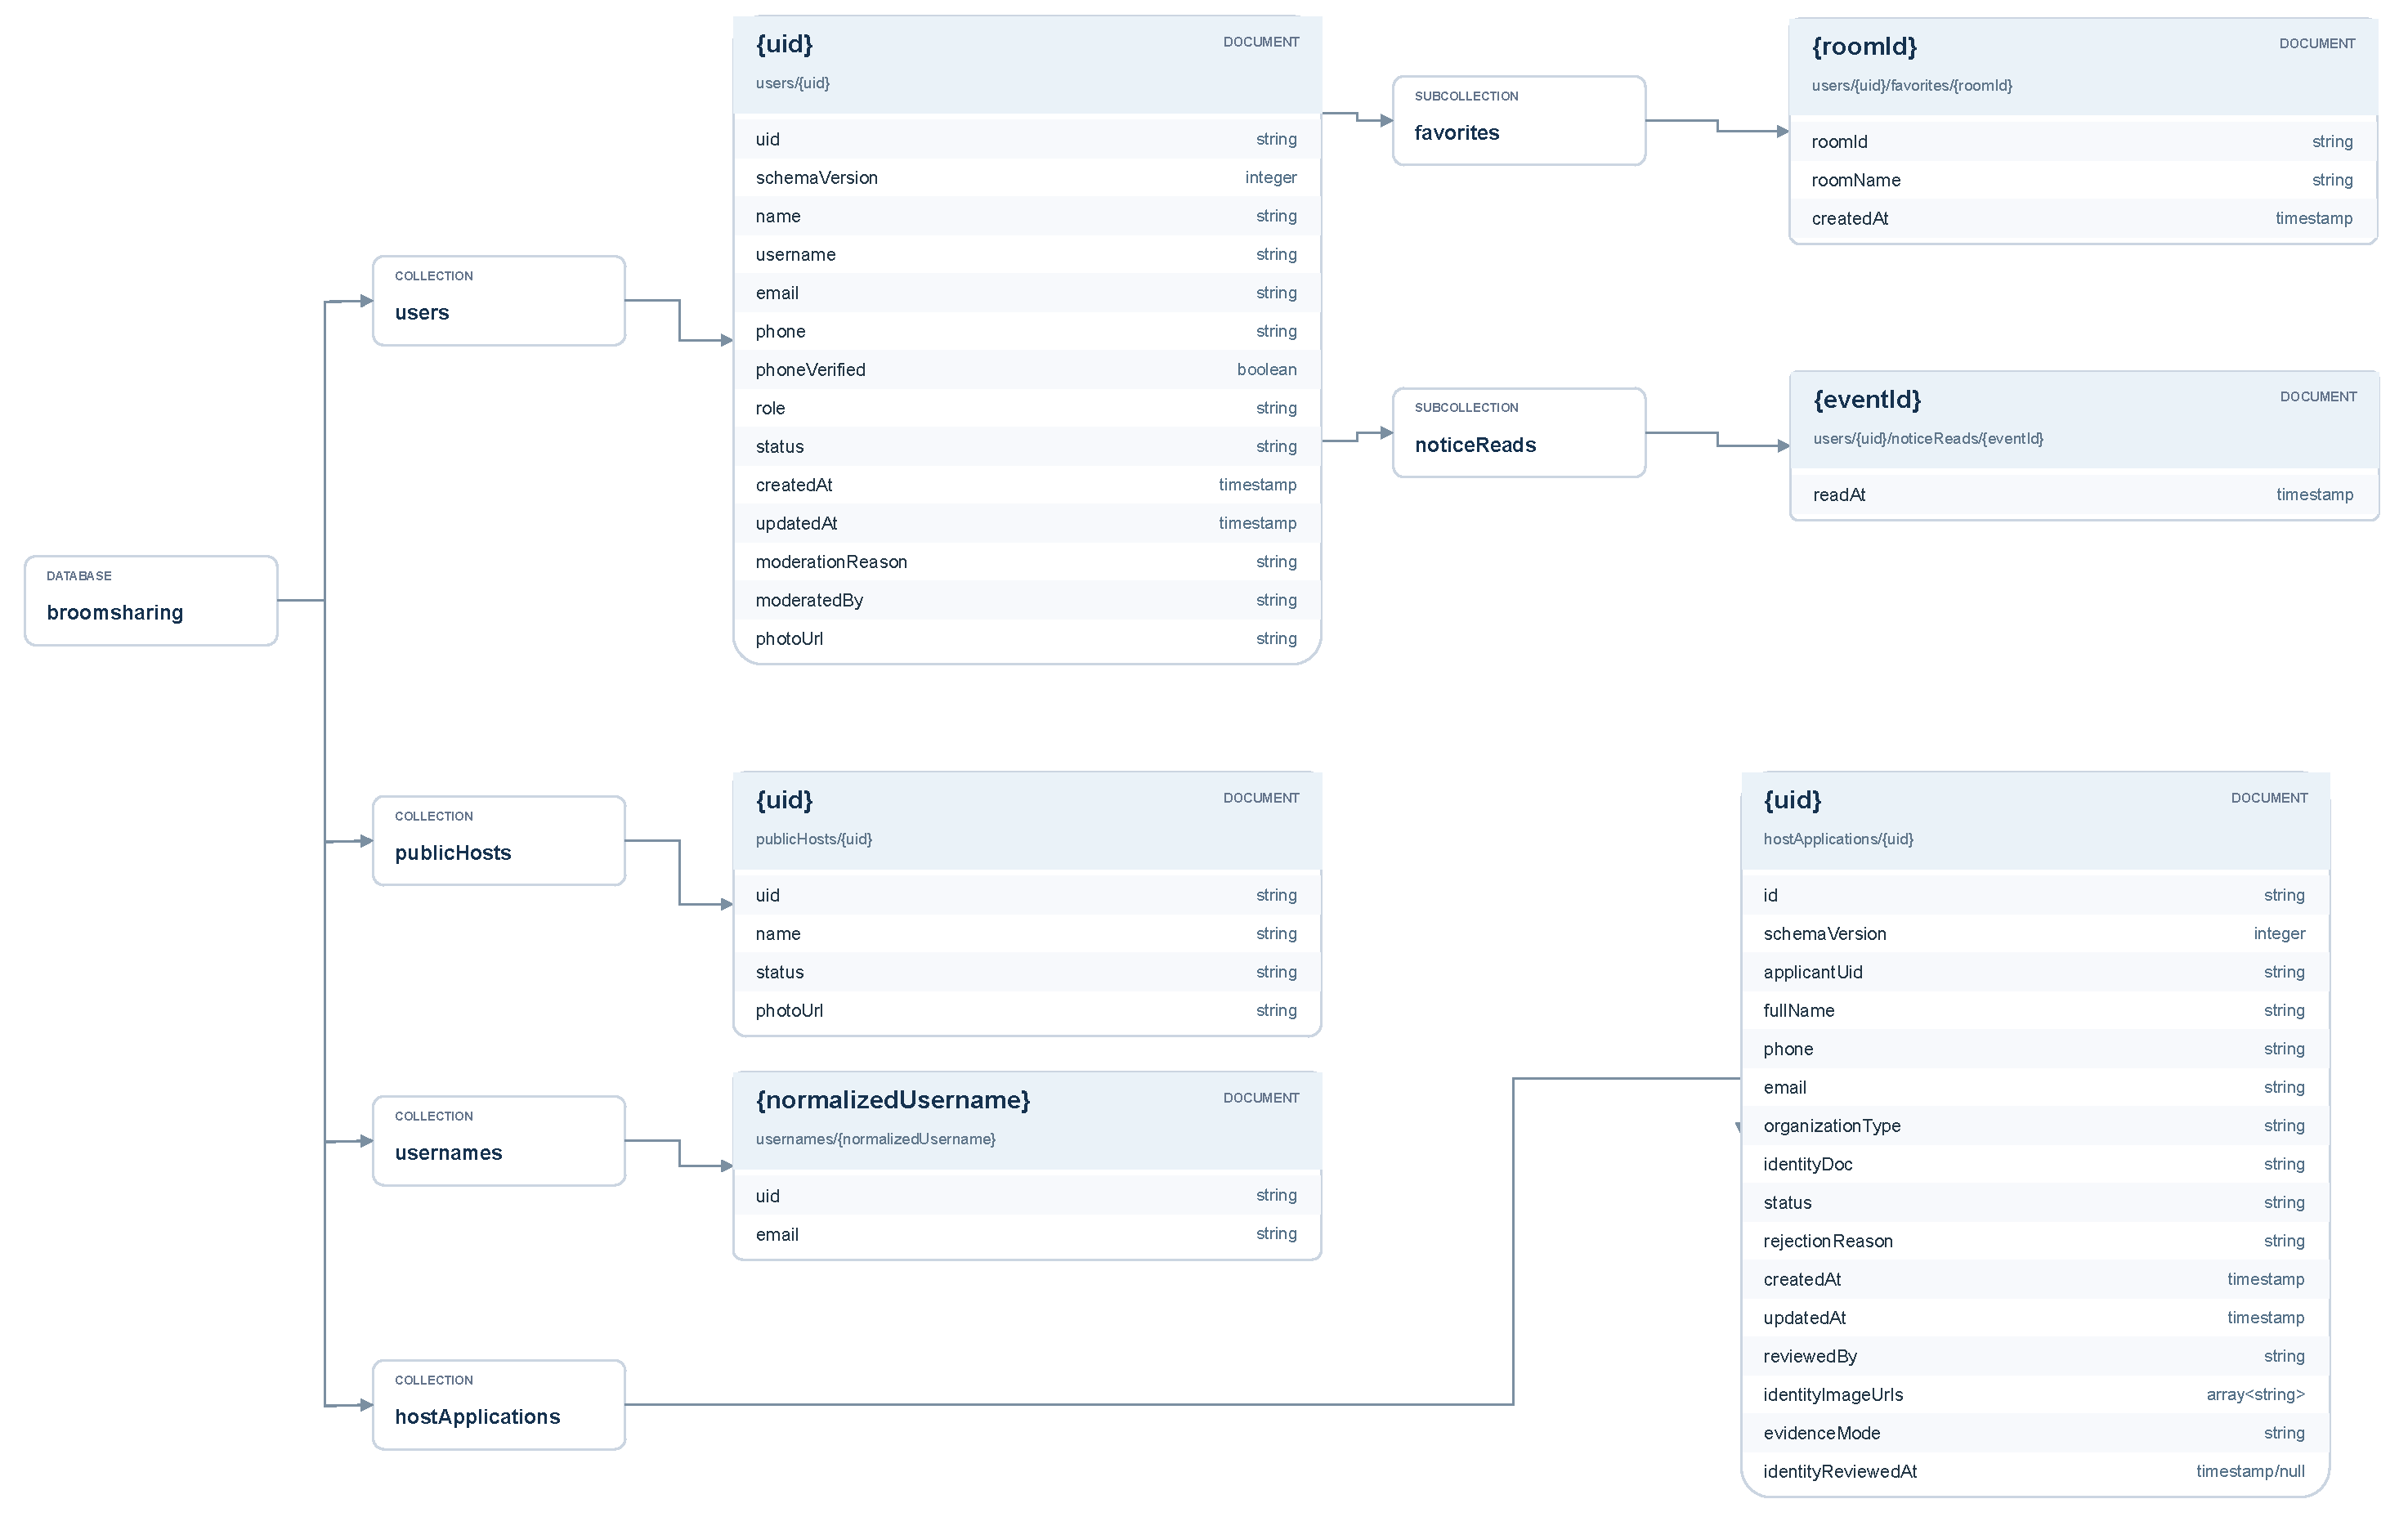
\includegraphics[width=\linewidth,height=0.82\textheight,keepaspectratio]{chapter4/firestore-accounts.pdf}
\caption{Cấu trúc nhóm tài khoản và các subcollection thuộc hồ sơ người dùng.}
\label{fig:ch4-accounts}
\end{figure}
\clearpage
\begin{figure}[p]
\centering
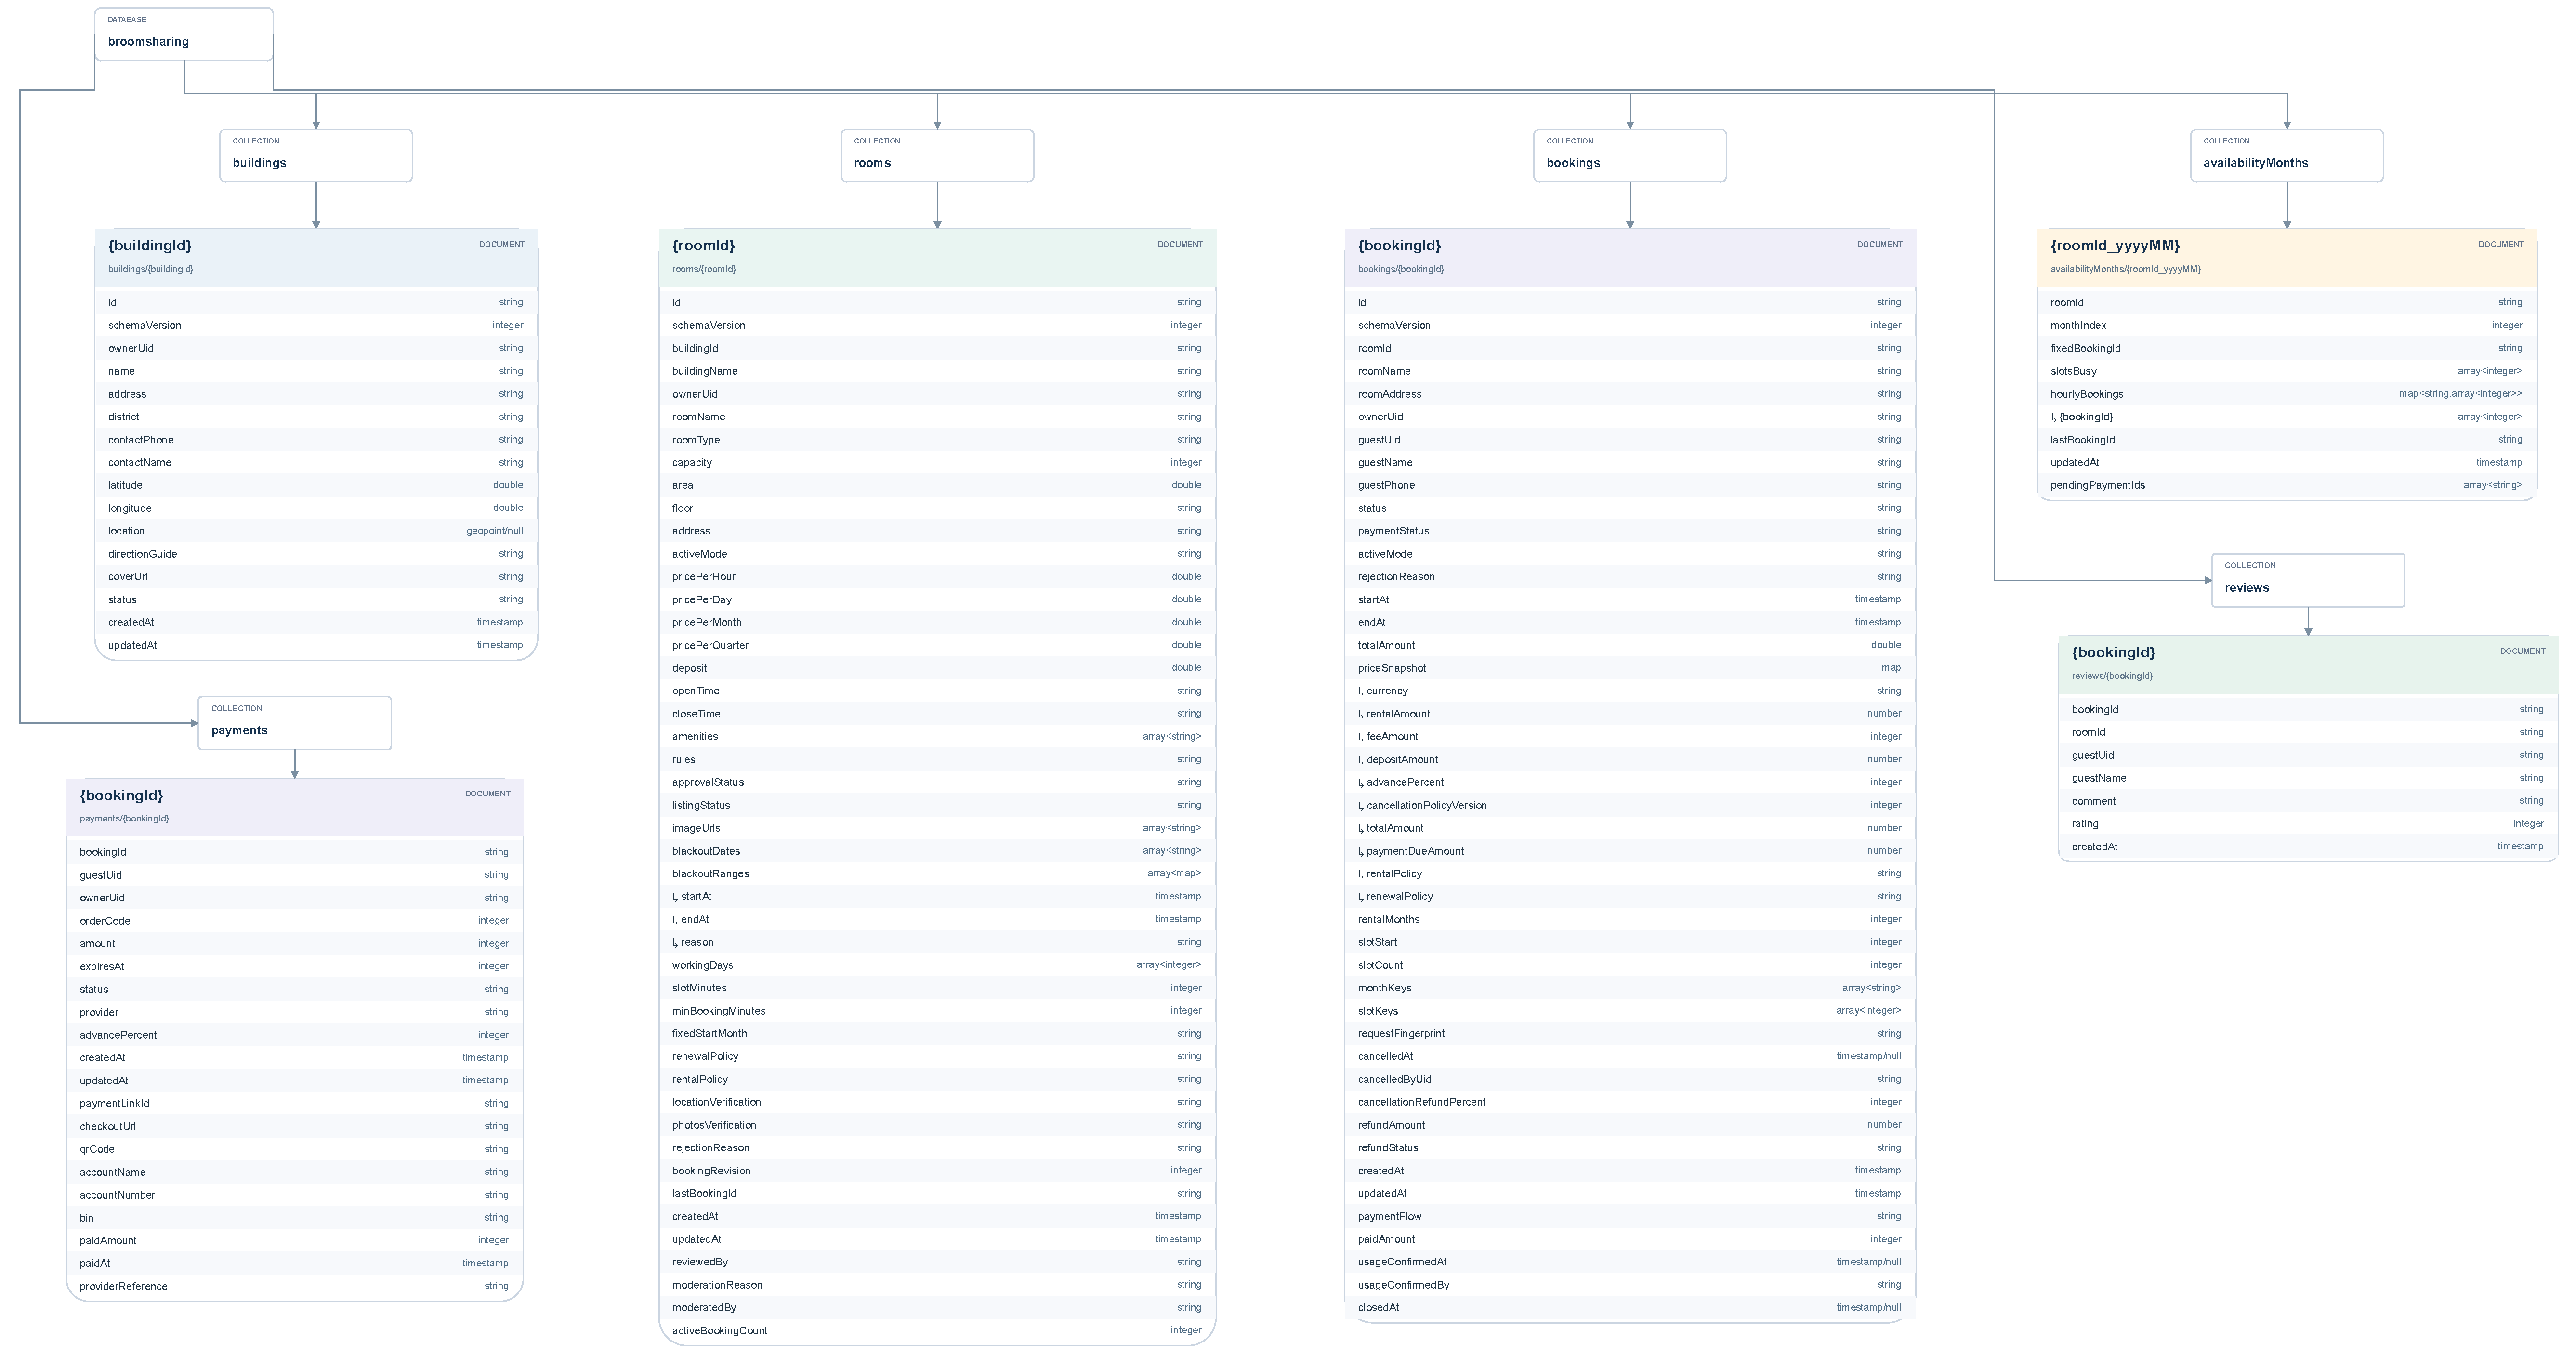
\includegraphics[width=\linewidth,height=0.82\textheight,keepaspectratio]{chapter4/firestore-booking.pdf}
\caption{Cấu trúc tài sản, booking, lịch tháng, thanh toán và đánh giá. Các collection nằm ngang cấp trong database.}
\label{fig:ch4-booking}
\end{figure}
\clearpage
\begin{figure}[p]
\centering
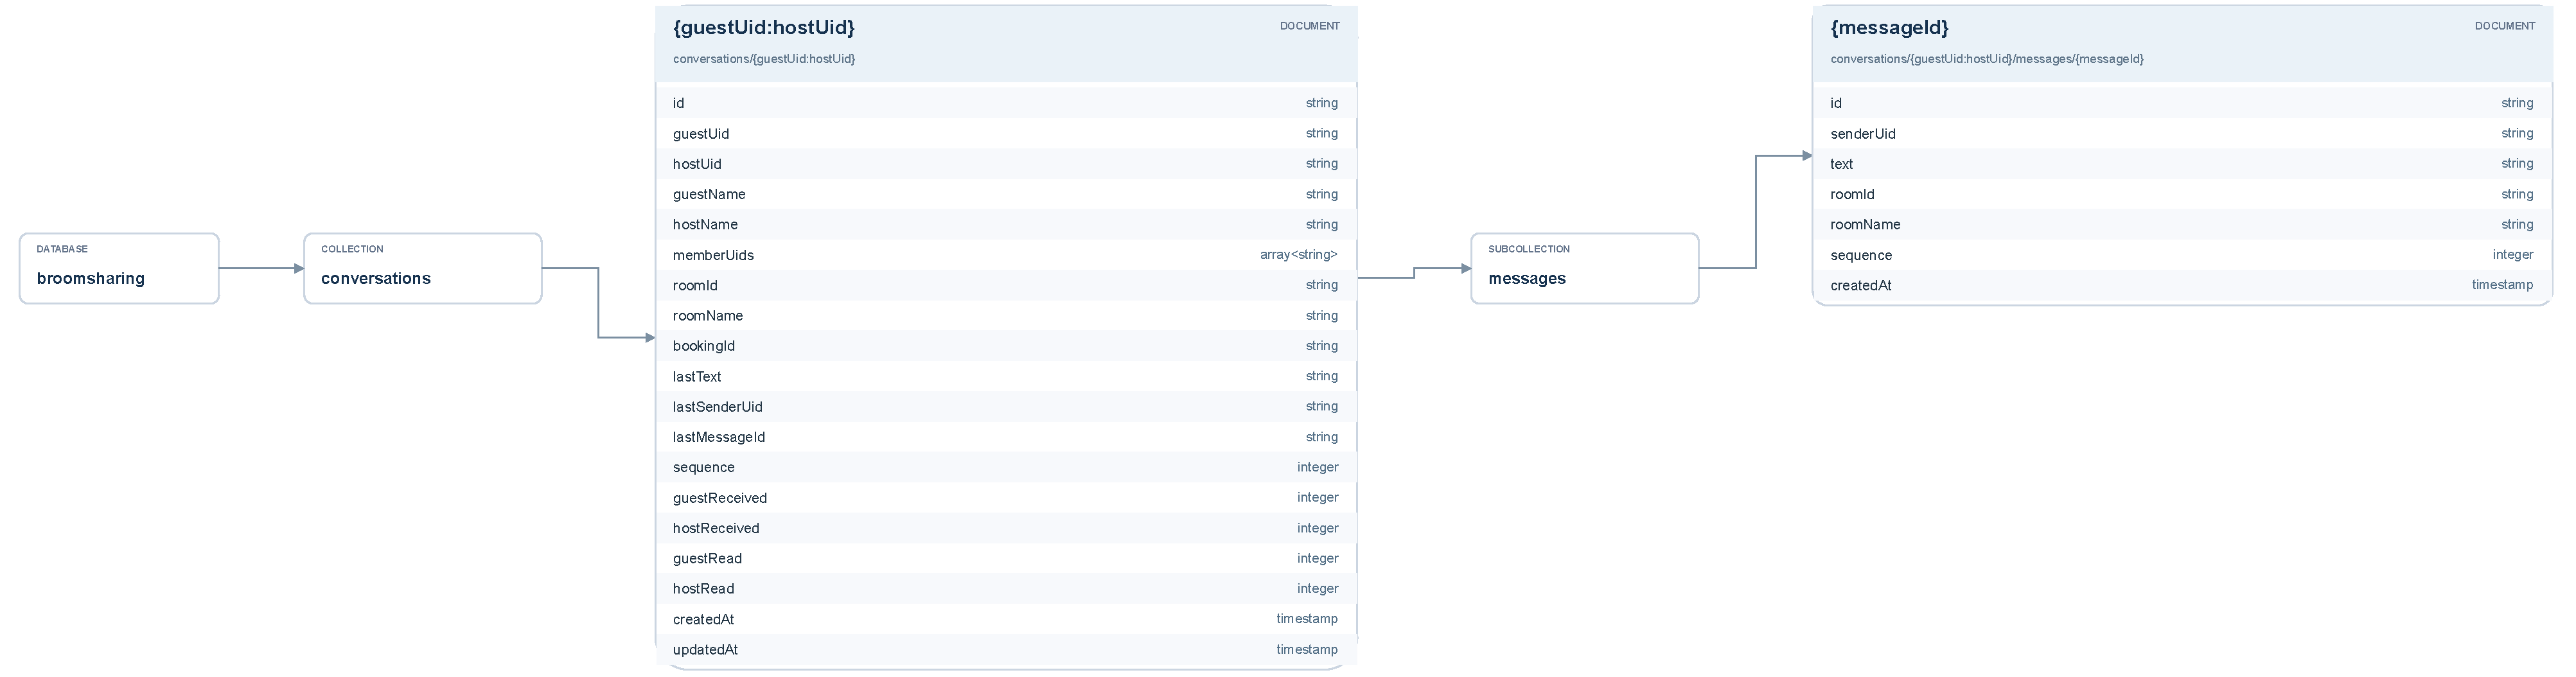
\includegraphics[width=\linewidth,height=0.82\textheight,keepaspectratio]{chapter4/firestore-chat.pdf}
\caption{Cấu trúc hội thoại và subcollection tin nhắn của từng hội thoại.}
\label{fig:ch4-chat}
\end{figure}
\clearpage
\begin{figure}[p]
\centering
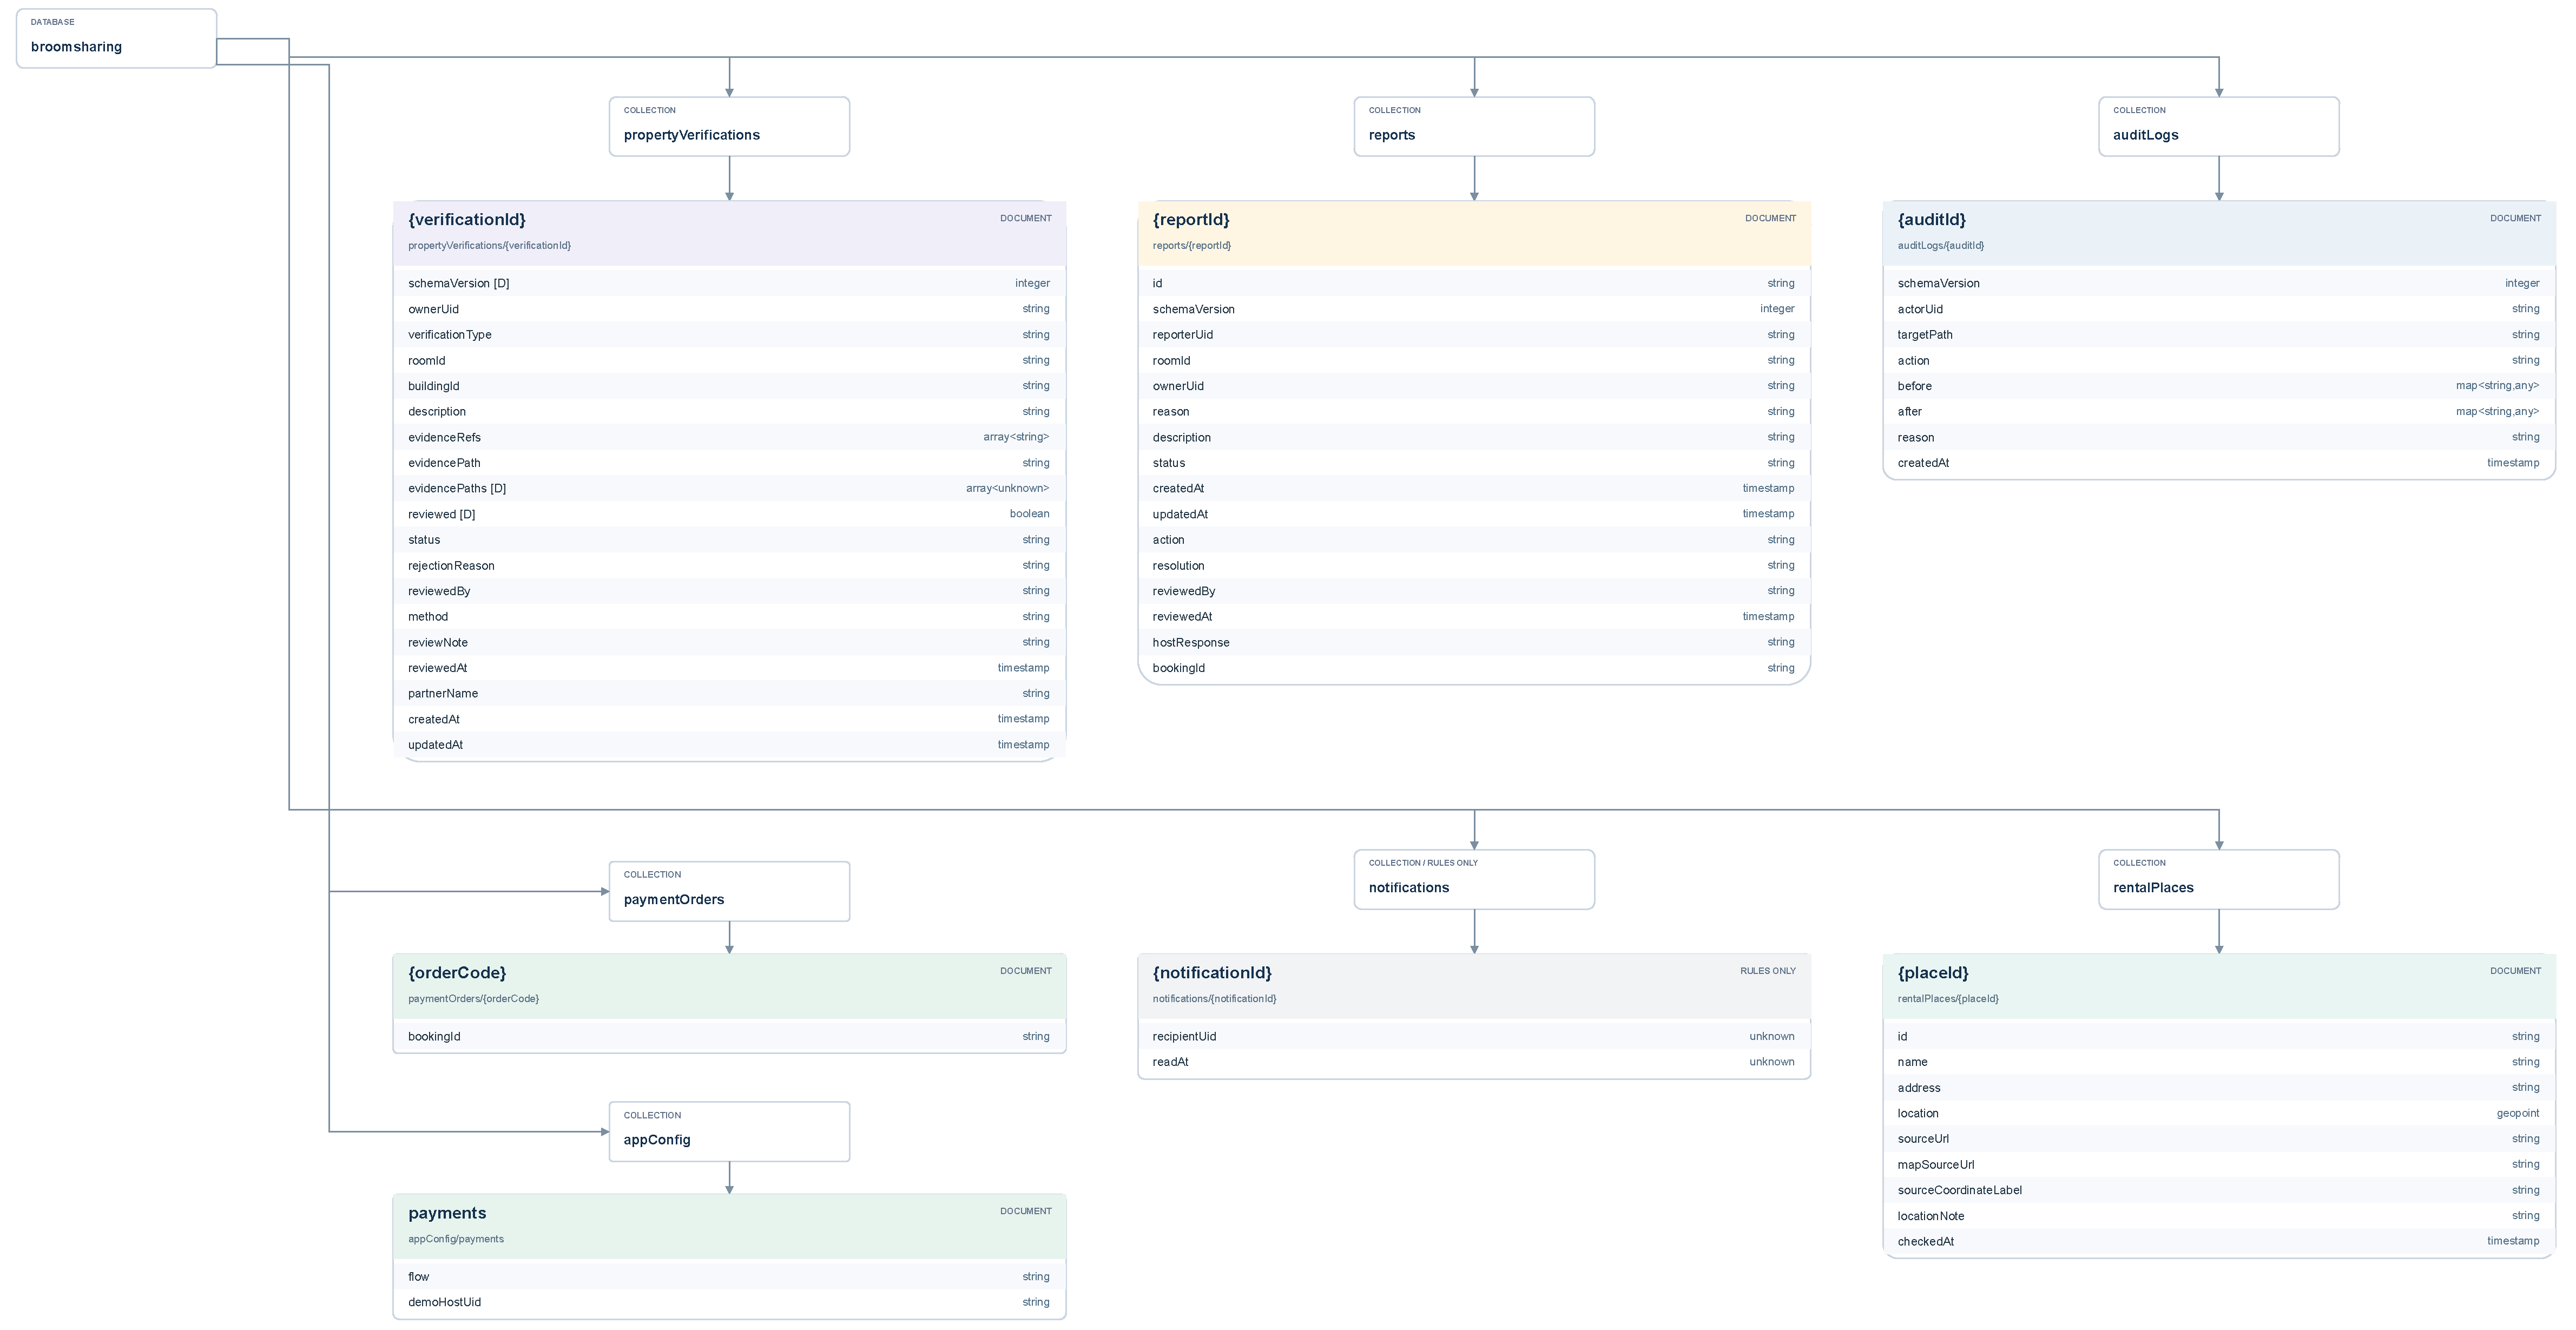
\includegraphics[width=\linewidth,height=0.82\textheight,keepaspectratio]{chapter4/firestore-administration.pdf}
\caption{Nhóm quản trị, dữ liệu tham khảo và cấu hình backend. [D] là trường từ dữ liệu mẫu; Rules-only là contract chưa có luồng ghi hiện tại.}
\label{fig:ch4-administration}
\end{figure}
\clearpage
\BroomLandscapePagefalse
\end{landscape}


Nhóm tài khoản trong Hình~\ref{fig:ch4-accounts} dùng chung UID để liên kết hồ sơ, bản chiếu Host và đơn đăng ký. Nhóm đặt chỗ trong Hình~\ref{fig:ch4-booking} liên kết tài sản với booking và lịch tháng bằng ID. Trong nhóm chat, mỗi document hội thoại sở hữu một subcollection tin nhắn riêng (Hình~\ref{fig:ch4-chat}); dữ liệu xác minh, báo cáo và nhật ký lưu thêm ID hoặc đường dẫn của đối tượng được xử lý (Hình~\ref{fig:ch4-administration}). Các liên kết logic này có ý nghĩa và bội số như Bảng~\ref{tab:ch4-relations-summary}.

\begingroup\small\setstretch{1.08}
\begin{longtable}{@{}>{\raggedright\arraybackslash}p{4.2cm}>{\raggedright\arraybackslash}p{5.15cm}>{\raggedright\arraybackslash}p{5.9cm}@{}}
\caption{Các quan hệ logic chính}\label{tab:ch4-relations-summary}\\
\toprule Nhóm dữ liệu & Liên kết & Ý nghĩa và bội số \\ \midrule\endfirsthead
\toprule Nhóm dữ liệu & Liên kết & Ý nghĩa và bội số \\ \midrule\endhead
\bottomrule\endlastfoot
Tài khoản & UID của hồ sơ, alias và bản chiếu Host. & Một User có một alias theo luồng đăng ký và tối đa một bản chiếu Host; UID liên kết với Authentication. \\
Tài sản & \texttt{rooms.\allowbreak{}building\allowbreak{}Id}; owner UID của Room và Building. & Một Building có nhiều Room; mỗi Room gắn với một Building và Host sở hữu tương ứng. \\
Đặt chỗ & Room ID, guest UID, owner UID. & Mỗi Booking thuộc một Room và hai bên tham gia; một Room có nhiều booking qua thời gian. \\
Lịch tháng & Room ID; fixed booking ID; khóa booking trong \texttt{hourly\allowbreak{}Bookings}. & Mỗi Room có nhiều tháng lịch; một tháng giữ toàn bộ cho một booking cố định hoặc giữ các slot thuê giờ. \\
Yêu thích & Room ID trong nhánh của User. & Quan hệ nhiều với nhiều giữa User và Room thông qua Favorite. \\
Hội thoại & \texttt{member\allowbreak{}Uids}; Room ID, Booking ID; sender UID của message. & Hai thành viên trong một hội thoại; một hội thoại có nhiều message và ngữ cảnh phòng hoặc booking. \\
Quản trị & UID chủ hồ sơ, người báo cáo, người duyệt; Room ID hoặc Building ID. & Hồ sơ xác minh và báo cáo liên kết tới đối tượng được xử lý; liên kết phụ thuộc loại hồ sơ. \\
Thanh toán & Booking ID của Payment; booking ID trong PaymentOrder. & Mỗi booking dùng một Payment cùng ID; order code ánh xạ về booking để đối soát webhook. Payment không phải subcollection của Booking.  \\
Nhật ký & Actor UID và \texttt{target\allowbreak{}Path}. & Actor xác định tài khoản hoặc tiến trình backend; đường dẫn đích thay đổi theo hành động. \\
\end{longtable}\endgroup

Map \texttt{price\allowbreak{}Snapshot} giữ giá và chính sách của booking; mảng \texttt{blackout\allowbreak{}Ranges} chứa các khoảng khóa lịch; map \texttt{hourly\allowbreak{}Bookings} ánh xạ booking ID tới tập slot. Đây là dữ liệu nhúng trong document. Room được thuê độc quyền trong khoảng $[startAt,endAt)$: PENDING giữ lịch tạm chờ thanh toán trong tối đa 5 phút, HOURLY dùng slot 30 phút và FIXED giữ trọn một hoặc ba tháng. Mảng \texttt{pending\allowbreak{}Payment\allowbreak{}Ids} phân biệt các khóa tạm chờ thanh toán với lịch đã xác nhận. Transaction duy trì sự nhất quán giữa booking, lịch tháng và revision của phòng.

\subsection{Một số thao tác dữ liệu tiêu biểu}
\label{sec:ch4-operations}

\subsubsection{Các nhóm thao tác dữ liệu}

Các Repository thực hiện ba nhóm thao tác: đọc dữ liệu theo điều kiện, theo dõi thay đổi bằng listener và ghi dữ liệu nghiệp vụ. Truy vấn danh sách giới hạn phạm vi theo trạng thái hoặc UID; listener cập nhật booking và trao đổi giữa hai bên; transaction xử lý những thay đổi liên quan nhiều document. Bảng~\ref{tab:ch4-operations} tổng hợp các thao tác tiêu biểu và dữ liệu tham gia.

\begingroup\small\setstretch{1.08}
\begin{longtable}{@{}>{\raggedright\arraybackslash}p{3.45cm}>{\raggedright\arraybackslash}p{4.25cm}>{\raggedright\arraybackslash}p{7.55cm}@{}}
\caption{Các thao tác dữ liệu tiêu biểu trong ứng dụng}\label{tab:ch4-operations}\\
\toprule Thao tác & Dữ liệu & Cách xử lý trong Repository \\ \midrule\endfirsthead
\toprule Thao tác & Dữ liệu & Cách xử lý trong Repository \\ \midrule\endhead
\midrule\multicolumn{3}{r}{\small Còn tiếp ở trang sau}\\\endfoot
\bottomrule\endlastfoot
Tải danh sách phòng & \texttt{rooms}; bổ sung Building và PublicHost. & Lọc APPROVED, ACTIVE; sắp theo document ID, lấy tối đa 20 phòng và phân trang bằng con trỏ. \\
Theo dõi booking & \texttt{bookings}. & Lọc \texttt{guest\allowbreak{}Uid} hoặc \texttt{owner\allowbreak{}Uid} theo tài khoản; nhận thay đổi qua listener. \\
Đọc lịch phòng & \texttt{availability\allowbreak{}Months}. & Đọc các document tháng liên quan để xác định lịch giữ chỗ theo giờ hoặc theo tháng. \\
Tạo booking & Booking, lịch tháng, Room và AuditLog. & Đọc và kiểm tra trong transaction; ghi booking PENDING cùng khóa lịch, revision phòng và nhật ký. \\
Chuyển trạng thái booking & Booking, lịch tháng, Room và AuditLog. & Kiểm tra bên thực hiện, trạng thái và thời gian; hủy, hết hạn hoặc khép lượt giải phóng khóa lịch tương ứng; booking mới được backend xác nhận sau thanh toán. \\
Đối soát thanh toán & Payment, Booking, lịch tháng, Room và AuditLog. & Backend kiểm tra kết quả payOS; xác nhận khi nhận đủ tiền đúng hạn hoặc khép link chưa trả và nhả lịch, không tự hoàn tiền.  \\
Theo dõi chat & \texttt{conversations} và subcollection \texttt{messages}. & Inbox lọc UID trong \texttt{member\allowbreak{}Uids}; tin nhắn sắp theo \texttt{sequence}, giới hạn số lượng và nhận cập nhật qua listener. \\
Gửi tin nhắn & Message và document hội thoại cha. & Transaction ghi tin, cập nhật preview, thứ tự và bộ đếm nhận tin của bên còn lại. \\
Lưu phòng yêu thích & \texttt{users/\allowbreak{}\{uid\}/\allowbreak{}favorites/\allowbreak{}\{room\allowbreak{}Id\}}. & Ghi ID, tên phòng và thời điểm lưu; bỏ yêu thích bằng cách xóa document tại cùng đường dẫn. \\
\end{longtable}\endgroup

Thao tác đọc danh sách và theo dõi thay đổi phục vụ hai nhu cầu khác nhau. Danh sách phòng được tải theo từng trang, còn booking và chat cần phản ánh cập nhật trong quá trình sử dụng. Các listener này bỏ qua snapshot từ cache hoặc còn ghi đang chờ xác nhận, thông qua metadata \texttt{isFrom\allowbreak{}Cache()} và \texttt{hasPending\allowbreak{}Writes()} \parencite{firebase_listeners}.

\Needspace{15\baselineskip}
\subsubsection{Các truy vấn tiêu biểu}

Khi tải danh sách không gian, \texttt{Room\allowbreak{}Repository.\allowbreak{}page()} chỉ chọn phòng đã duyệt APPROVED và đang hiển thị ACTIVE. Tham số \texttt{after} là document ID cuối của lượt tải trước; ở lượt đầu, tham số này bằng \texttt{null}. Truy vấn sắp xếp theo document ID và giới hạn bằng hằng \texttt{PAGE\_SIZE=20}; \texttt{start\allowbreak{}After()} đặt điểm bắt đầu cho lượt tiếp theo \parencite{firebase_queries,firebase_query_cursors}.

\par\medskip\noindent\begin{minipage}{\linewidth}
\inputminted[firstnumber=1]{java}{Resources/chapter4/code/room-query.java}
{\footnotesize\noindent Nguồn: \texttt{Room\allowbreak{}Repository.\allowbreak{}java}, dòng 63 đến 70.\par}
\end{minipage}\par\medskip

Kết quả được đọc từ máy chủ bằng \texttt{get(Source.\allowbreak{}SERVER)}. Repository lấy ID của document cuối làm con trỏ, rồi đọc bổ sung Building và PublicHost để tạo danh sách \texttt{Room\allowbreak{}Listing}. Khi không có document, con trỏ giữ giá trị trước đó. Cờ \texttt{hasMore} được đặt theo điều kiện số document bằng 20; đây là căn cứ cho phép thử tải tiếp, chưa khẳng định lượt kế tiếp chắc chắn còn dữ liệu. Lỗi truy vấn được chuyển tới callback lỗi, tách khỏi trường hợp truy vấn thành công nhưng danh sách rỗng.

\texttt{Room\allowbreak{}ViewModel} gọi \texttt{page()}, cập nhật con trỏ và ghép kết quả theo Room ID để tránh trùng phòng. Khi có từ khóa hoặc bộ lọc, ViewModel tự tải các trang còn lại trước khi kết luận không có kết quả; danh sách được phát qua \texttt{LiveData}; \texttt{Main\allowbreak{}Activity} quan sát kết quả để cập nhật danh sách và nút tải thêm.

Với danh sách booking, \texttt{Booking\allowbreak{}Repository.\allowbreak{}watchMine()} lọc \texttt{guest\allowbreak{}Uid} bằng UID hiện tại qua hàm dùng chung \texttt{watch\allowbreak{}Participant()}. Listener nhận thay đổi từ Firestore và chỉ chuyển snapshot đã được máy chủ xác nhận tới callback. Các document được ánh xạ thành \texttt{Booking}, sắp theo thời điểm tạo booking giảm dần rồi trả về ViewModel.

\par\medskip\noindent\begin{minipage}{\linewidth}
\inputminted[firstnumber=1]{java}{Resources/chapter4/code/booking-query-listener.java}
{\footnotesize\noindent Nguồn: \texttt{Booking\allowbreak{}Repository.\allowbreak{}java}, dòng 659 đến 671.\par}
\end{minipage}\par\medskip

\texttt{Booking\allowbreak{}ViewModel.\allowbreak{}watchMine()} đặt trạng thái tải, gọi Repository và cập nhật \texttt{bookings} bằng \texttt{UiState.\allowbreak{}success()} hoặc \texttt{UiState.\allowbreak{}error()}. \texttt{My\allowbreak{}Bookings\allowbreak{}Activity} quan sát \texttt{LiveData} này để hiển thị dữ liệu và lọc trạng thái tại giao diện. Khi màn hình dừng, listener được gỡ; khi hiển thị lại, truy vấn được đăng ký lại để nhận các thay đổi tiếp theo.

\subsubsection{Tạo booking bằng transaction}

Khi người thuê gửi yêu cầu, \texttt{Booking\allowbreak{}Repository.\allowbreak{}create()} phải xác nhận phòng còn nhận đặt và khoảng thuê chưa bị chiếm. Booking ID được băm từ UID cùng \texttt{request\allowbreak{}Key}; trường \texttt{request\allowbreak{}Fingerprint} biểu diễn nội dung yêu cầu. Nếu document theo ID này đã tồn tại và fingerprint trùng khớp, phương thức trả lại booking ID cũ. Nếu fingerprint khác, yêu cầu bị từ chối, tránh dùng lại cùng mã gửi cho một lựa chọn khác.

Trong callback \texttt{run\allowbreak{}Transaction()}, Repository đọc hồ sơ người thuê, phòng, bản chiếu Host, tòa nhà, cấu hình \texttt{appConfig/payments} và các tháng lịch liên quan. Booking mới phải thuộc Host của kênh demo với luồng \texttt{INSTANT\_5M}. Tài khoản phải ACTIVE và có vai trò GUEST hoặc HOST; phòng phải APPROVED, ACTIVE và không thuộc chính người thuê. Host cùng tòa nhà phải còn hoạt động, đồng thời owner UID của Room phải khớp Building. Giá và thời gian thuê được tính lại từ dữ liệu phòng bằng \texttt{Booking\allowbreak{}Policy.\allowbreak{}plan()}, sau đó lịch được kiểm tra trước mọi lệnh ghi.

\par\medskip\noindent\begin{minipage}{\linewidth}
\inputminted[firstnumber=1]{java}{Resources/chapter4/code/booking-prepare.java}
{\footnotesize\noindent Nguồn: \texttt{Booking\allowbreak{}Repository.\allowbreak{}java}, dòng 206 đến 217.\par}
\end{minipage}\par\medskip

Hàm \texttt{months()} đọc lịch tháng bằng chính transaction. Với thuê giờ, \texttt{reserve()} kiểm tra tập slot mới không giao với \texttt{slotsBusy}; với thuê cố định, tháng phải chưa có booking cố định hoặc booking giờ. Nếu có xung đột, hàm phát sinh lỗi trước bước ghi. Khi hợp lệ, các đối tượng lịch được cập nhật trong bộ nhớ rồi ghi cùng booking, revision của phòng và nhật ký.

\par\medskip\noindent\begin{minipage}{\linewidth}
\inputminted[firstnumber=1]{java}{Resources/chapter4/code/booking-commit.java}
{\footnotesize\noindent Nguồn: \texttt{Booking\allowbreak{}Repository.\allowbreak{}java}, dòng 226 đến 237.\par}
\end{minipage}\par\medskip

Firestore áp dụng toàn bộ các lệnh ghi trong transaction theo tính nguyên tử và có thể chạy lại callback khi document đã đọc bị thay đổi đồng thời \parencite{firebase_transaction}. Vì các yêu cầu cùng phòng đọc và cập nhật lịch tháng chung, việc kiểm tra xung đột được thực hiện lại trên lịch mới khi transaction chạy lại. Callback thành công trả về booking ID sau khi giao dịch hoàn tất; lỗi kiểm tra, xung đột hoặc lỗi ghi được chuyển tới callback lỗi. Kết quả ghi thành công là booking PENDING và phần lịch tạm giữ; đây chưa phải xác nhận đã thanh toán. Màn hình QR được mở ngay để tiếp tục cùng booking.

Booking mới lưu \texttt{schema\allowbreak{}Version=\allowbreak{}2}, giá và chính sách tại thời điểm đặt trong \texttt{price\allowbreak{}Snapshot}. Trường \texttt{paymentFlow=INSTANT\_5M} xác định luồng giữ lịch tạm. Trước khi tạo yêu cầu payOS, booking chưa ghi nhận tiền; sau đó Payment theo dõi mã đơn, số tiền, QR và thời hạn. Backend đối chiếu kết quả nhà cung cấp, số tiền và thời điểm nhận tiền trước khi xác nhận \texttt{PAID/CONFIRMED}. Khi link đã kết thúc mà chưa trả tiền, backend chuyển booking sang \texttt{EXPIRED}, nhả đúng khóa lịch và giữ lịch sử. Tiền đến muộn, sai số tiền hoặc lịch không còn hợp lệ được đưa vào \texttt{REVIEW\_REQUIRED}; chưa có API hoàn tiền tự động.

\Needspace{8\baselineskip}
\subsection{Phân quyền và bảo vệ dữ liệu}
\label{sec:ch4-security}

Firestore Rules kết hợp UID, vai trò, trạng thái ACTIVE và quyền sở hữu để kiểm soát truy cập. Guest và Host đều có quyền thuê, nhưng không được tự đặt phòng của mình. Bảng~\ref{tab:ch4-permissions} tóm tắt các nhóm quyền chính; các thao tác ngoài nhánh được cho phép chịu quy tắc từ chối mặc định.

\begingroup\small\setstretch{1.08}
\begin{longtable}{@{}>{\raggedright\arraybackslash}p{4.1cm}>{\raggedright\arraybackslash}p{11.15cm}@{}}
\caption{Phân quyền theo nhóm dữ liệu}\label{tab:ch4-permissions}\\
\toprule Nhóm & Quyền truy cập chính \\ \midrule\endfirsthead
\toprule Nhóm & Quyền truy cập chính \\ \midrule\endhead
\bottomrule\endlastfoot
Hồ sơ và đơn Host & Chủ hồ sơ hoặc Admin được đọc. Người dùng sửa nhóm trường hồ sơ cho phép; Guest nộp đơn, Admin xét duyệt. PublicHost được đọc bởi tài khoản hoạt động. \\
Alias và dữ liệu cá nhân & \texttt{usernames} cho phép get trước đăng nhập, list chỉ dành cho Admin. Favorite và mốc đã đọc thuộc quyền tài khoản sở hữu nhánh dữ liệu. \\
Tòa nhà và phòng & Host quản lý tài sản của mình; Admin được cập nhật Room, không có nhánh ghi Building riêng. Phòng công khai cho tài khoản hoạt động khi APPROVED và ACTIVE. \\
Booking và lịch & Hai bên tham gia và Admin được đọc Booking. Chuyển trạng thái phụ thuộc vai trò, thời gian và lịch; Admin không có nhánh chuyển tùy ý. Ghi lịch phải khớp booking trong cùng thao tác. \\
Thanh toán và cấu hình & Người thuê, Host liên quan và Admin được đọc Payment; client không được tự ghi trạng thái tiền. PaymentOrder chỉ do backend truy cập; cấu hình kênh cho tài khoản hoạt động đọc, không chứa khóa payOS.  \\
Chat & Chỉ thành viên đang hoạt động đọc hội thoại và message. Gửi tin cập nhật đồng thời preview, thứ tự và bộ đếm; mỗi bên chỉ tăng mốc đã đọc của mình. Admin không có quyền đọc riêng. \\
Quản trị và tham khảo & Chủ hồ sơ hoặc Admin đọc xác minh; Admin cập nhật kết quả. Báo cáo được đọc theo người gửi, Host liên quan hoặc Admin. Audit chỉ Admin đọc; RentalPlace chỉ cho tài khoản hoạt động đọc. \\
\end{longtable}\endgroup

Quyền ghi còn phụ thuộc nội dung và tính nhất quán giữa document. Rules dùng danh sách trường cho phép và \texttt{diff().\allowbreak{}affected\allowbreak{}Keys()} để giới hạn thay đổi; \texttt{get\allowbreak{}After()} kiểm tra trạng thái sau ghi của các document liên quan \parencite{firebase_rules_fields,firebase_rules_conditions}. Ví dụ, \texttt{held\allowbreak{}Month()} đối chiếu booking với lịch tháng trước khi chấp nhận thao tác giữ chỗ.

\par\medskip\noindent\begin{minipage}{\linewidth}
\inputminted[firstnumber=1]{text}{Resources/chapter4/code/rules-held-month.txt}
{\footnotesize\noindent Nguồn: \texttt{firestore.\allowbreak{}rules}, dòng 24 đến 30.\par}
\end{minipage}\par\medskip

Backend dùng Firebase Admin SDK nên phải tự xác thực Firebase ID token, kiểm tra người tham gia và đối chiếu kết quả payOS; không dựa vào Rules để xác thực lệnh ghi của server \parencite{firebase_rules_conditions}. Khóa dịch vụ được giữ ở môi trường backend. Ảnh và minh chứng DEMO hiện dùng URL Cloudinary; Rules kiểm tra đường dẫn theo UID và đối tượng liên quan. Ảnh giấy tờ DEMO công khai theo URL không được xem là cơ chế bảo vệ giấy tờ cá nhân thật.

\endgroup
